% Created 2014-02-25 Di 21:55
\documentclass[11pt]{article}
\usepackage[utf8]{inputenc}
\usepackage[T1]{fontenc}
\usepackage{fixltx2e}
\usepackage{graphicx}
\usepackage{longtable}
\usepackage{float}
\usepackage{wrapfig}
\usepackage{soul}
\usepackage{textcomp}
\usepackage{marvosym}
\usepackage{wasysym}
\usepackage{latexsym}
\usepackage{amssymb}
\usepackage{hyperref}
\tolerance=1000
\providecommand{\alert}[1]{\textbf{#1}}

\title{README}
\author{Michael Klöckner}
\date{\today}
\hypersetup{
  pdfkeywords={},
  pdfsubject={},
  pdfcreator={Emacs Org-mode version 7.8.11}}

\begin{document}

\maketitle

\setcounter{tocdepth}{3}
\tableofcontents
\vspace*{1cm}


\section{Overview}
\label{sec-1}
\subsection{Purpose}
\label{sec-1-1}

This paper documents the Proof of Concept Project:
\textbf{Enable a Jenkins build server to publish release artifacts as} \emph{Docker} \textbf{images to a} \emph{Docker} \textbf{reegistry. Start service on a new EC2 node by fetching the artifact from the registry.}
\subsection{Author}
\label{sec-1-2}

\begin{itemize}
\item Author: Michael Klöckner, Weberstr. 39, 60318 Frankfurt am Main,
\item Email:mkl@im7.de
\item Phone: +49 69 9866 1103
\end{itemize}
\subsection{\emph{Docker} version}
\label{sec-1-3}

   We installed \emph{Docker} version 0.8 in 2014/02.
\subsection{Deployment workflow}
\label{sec-1-4}

One major issue in Continuous Integration is to insure a once deployed build artifact never changes in future deployment scenarios. \emph{Docker} versions each container, making it immutable after a \texttt{docker build}. To start a particular container, beeing pulled out of a repository, results in starting the same build artifact in all future deployment scenarios. We use the \emph{Jenkins} server to build a docker container triggered by a git push. This container is then pulled and started by the production environment.
\href{file:///debiandata/michael/elemica/docker/poc-docker-jenkins/img/docker-deployment-workflow-01.jpg}{docker-deployment-workflow-01.jpg}
\section{\emph{Docker}}
\label{sec-2}

This chapter deals with installation issues and some basic \emph{Docker} commands. It is mainly take from the \href{http://docs.docer.io/en/latest/}{Docker documentation}. 
\subsection{\textbf{TODO} explain \emph{docker} terminology: Image, Container, Repository, Registry, Index.}
\label{sec-2-1}
\subsection{Installation}
\label{sec-2-2}
\subsubsection{Kernel options}
\label{sec-2-2-1}

\emph{Docker} needs a 64-Bit Linux distribution, a recent kernel > 3.8 and LXC
installed. Either you use a system with the appropriate kernel installed, or
you update the kernel by hand as described in kernel compilation. The kernel needs to have compiled all options concerning virtual NICs, especially
BRIDGED NICs, all NAT options and all net  ( NF ) options. Download
the kernel source, untar it, change into the directory and configure it properly. To compile the kernel as a debian package named \textbf{fora-kernel-3.13.3}
to be installed later together with it's header follow these instructions:

\begin{verbatim}
make-kpkg clean
make-kpkg --append-to-version "-flora-kernel-3.13.3" --revision "1" \
--initrd kernel_image kernel_headers
\end{verbatim}
The package is to be found one directory upwards and can be installed using

\begin{verbatim}
dpkg -i ../linux-headers-3.13.3-flora-kernel-3.13.3_1.2_amd64.deb \
../linux-image-3.13.3-flora-kernel-3.13.3_1.2_amd64.deb/.
\end{verbatim}
\subsubsection{Installation by hand}
\label{sec-2-2-2}

First add the \emph{Docker} repository key to your local keychain.

\begin{verbatim}
sudo apt-key adv --keyserver keyserver.ubuntu.com \
--recv-keys 36A1D7869245C8950F966E92D8576A8BA88D21E9
\end{verbatim}
Add the \emph{Docker} repository to your apt sources list, update and install
the lxc-docker package.

\begin{verbatim}
sudo sh -c "echo deb http://get.docker.io/ubuntu docker main\
> /etc/apt/sources.list.d/docker.list"
sudo apt-get update
sudo apt-get install lxc-docker
\end{verbatim}
Now verify that the installation has worked by downloading the ubuntu
image and launching a container. \texttt{sudo docker run -i -t ubuntu /bin/bash}.
Type exit to exit.
\subsubsection{Installation by script}
\label{sec-2-2-3}

Docker.io provides an installation script to be called: \texttt{curl -s https://get.docker.io/ubuntu/ | sudo sh}
Now verify that the installation has worked by downloading the ubuntu
image and launching a container. \texttt{sudo docker run -i -t ubuntu /bin/bash}
Type exit to exit.
\subsubsection{Installing on AWS}
\label{sec-2-2-4}

Docker.io provides an installation guide for Amazon Web Services EC2.
\begin{itemize}
\item Choose an image:
\begin{itemize}
\item Launch the Create Instance Wizard menu on your AWS Console.
\item Click the Select button for a 64Bit Ubuntu image. For example: Ubuntu Server 12.04.3 LTS.
\item For testing you can use the default (possibly free) t1.micro instance (more info on pricing).
\item Click the Next: Configure Instance Details button at the bottom right.
\end{itemize}
\item Tell CloudInit to install \emph{Docker}:
\begin{itemize}
\item When you're on the Configure Instance Details step, expand the Advanced Details section.
\item Under User data, select As text
\item Enter \#include \href{https://get.docker.io}{https://get.docker.io}  into the instance User Data. CloudInit is part of the Ubuntu image you chose; it will bootstrap \emph{Docker} by running the shell script located at this URL.
\end{itemize}
\item After a few more standard choices where defaults are probably OK, your AWS Ubuntu instance with \emph{Docker} should be running!
\end{itemize}
If this is your first AWS instance, you may need to set up your Security Group to allow SSH. By default all incoming ports to your new instance will be blocked by the AWS Security Group, so you might just get
timeouts when you try to connect. Installing with get.docker.io (as above) will create a service named lxc-
docker. It will also set up a \emph{docker} group and you may want to add the ubuntu user to it so that you don't have to use sudo for every \emph{Docker} command.
\subsubsection{Configuration}
\label{sec-2-2-5}

\begin{itemize}
\item The daemon's config file is placed in \emph{etc/default/docker}.
\item Images, containers and their configurations are placed under \emph{var/lib/docker}.
\end{itemize}
\subsection{Play with \emph{Docker}}
\label{sec-2-3}

We describe some basic \emph{Docker} commands.
\subsubsection{Check your \emph{Docker} installation.}
\label{sec-2-3-1}


\begin{verbatim}
# Check that you have a working install
docker info
\end{verbatim}
\subsubsection{Download a pre-built image}
\label{sec-2-3-2}


\begin{verbatim}
# Download an ubuntu image
sudo docker pull ubuntu
\end{verbatim}
\subsubsection{Run an interactive shell}
\label{sec-2-3-3}


\begin{verbatim}
# Run an interactive shell in the ubuntu image,
# allocate a tty, attach stdin and stdout
# To detach the tty without exiting the shell,
# use the escape sequence Ctrl-p + Ctrl-q
sudo docker run -i -t ubuntu /bin/bash
\end{verbatim}
\subsubsection{Bind to a port}
\label{sec-2-3-4}

The \emph{Docker} client can use -H to connect to a custom port.
-H accepts host and port assignment in the following format: 
\begin{itemize}
\item tcp://[host][:port]  =
\item unix://path =
\item host[:port] or :port =
\end{itemize}


\begin{verbatim}
# Run docker in daemon mode
sudo <path to>/docker -H 0.0.0.0:5555 -d &
# Download an ubuntu image
sudo docker -H :5555 pull ubuntu
\end{verbatim}
\subsubsection{Starting a long run}
\label{sec-2-3-5}


\begin{verbatim}
# Start a very useful long-running process
JOB=$(sudo docker run -d ubuntu /bin/sh -c "while true; \
do echo Hello world; sleep 1; done")
# Collect the output of the job so far
sudo docker logs $JOB
# Kill the job
sudo docker kill $JOB
\end{verbatim}
\subsubsection{Bind a service on a TCP port}
\label{sec-2-3-6}


\begin{verbatim}
# Bind port 4444 of this container, and tell netcat to listen on it
JOB=$(sudo docker run -d -p 4444 ubuntu:12.10 /bin/nc -l 4444)

# Which public port is NATed to my container?
PORT=$(sudo docker port $JOB 4444 | awk -F: '{ print $2 }')

# Connect to the public port
echo hello world | nc 127.0.0.1 $PORT

# Verify that the network connection worked
echo "Daemon received: $(sudo docker logs $JOB)"
\end{verbatim}
\subsubsection{Committing (saving) a container state}
\label{sec-2-3-7}

Save your containers state to a container image, so the state can be re-used.
When you commit your container only the differences between the image the container was created from and the current state of the container will be stored (as a diff). See which images you already have using the \emph{Docker} images command.

\begin{verbatim}
# Commit your container to a new named image
sudo docker commit <container_id> <some_name>

# List your containers
sudo docker images
\end{verbatim}
\subsubsection{Committing a Container to a Named Image}
\label{sec-2-3-8}

When you make changes to an existing image, those changes get saved to a container’s file system. You can then promote that container to become an image by making a commit. In addition to converting the container to an image, this is also your opportunity to name the image, specifically a name that includes your user name from the Central \emph{Docker} Index (as you did a login above) and a meaningful name for the image.

\begin{verbatim}
# format is "sudo docker commit <container_id> <username>/<imagename>"
$ sudo docker commit $CONTAINER_ID myname/kickassapp
\end{verbatim}
\subsubsection{Pushing an image to its repository}
\label{sec-2-3-9}

In order to push an image to its repository you need to have committed your container to a named image (see above).
Now you can commit this image to the repository designated by its name or tag.

\begin{verbatim}
# format is "docker push <username>/<repo_name>"
$ sudo docker push myname/kickassapp
\end{verbatim}
\subsubsection{Export a container}
\label{sec-2-3-10}

To export a container to a tar file just type:

\begin{verbatim}
$ docker images
REPOSITORY          TAG                 IMAGE ID            CREATED             VIRTUAL SIZE
mkl/debian          7.4                 11ed3d47ec89        About an hour ago   117.8 MB
mkl/debian          latest              11ed3d47ec89        About an hour ago   117.8 MB
mkl/debian          wheezy              11ed3d47ec89        About an hour ago   117.8 MB
ubuntu              13.10               9f676bd305a4        2 weeks ago         182.1 MB
ubuntu              saucy               9f676bd305a4        2 weeks ago         182.1 MB

$ docker ps -a
CONTAINER ID        IMAGE               COMMAND             CREATED             STATUS              PORTS               NAMES
ac3a595c294c        mkl/debian:7.4      /bin/bash           58 minutes ago      Exit 1                                  prickly_lovelace    
f7528d270208        mkl/debian:7.4      echo success        About an hour ago   Exit 0                                  jovial_pare         
6a569d77e974        ubuntu:12.04        /bin/bash           16 hours ago        Exit 0                                  backstabbing_pike 

$ docker export ac3a595c294c  > exampleimage.tar
\end{verbatim}
\subsubsection{Import a container}
\label{sec-2-3-11}

At this time, the URL must start with http and point to a single file archive (.tar, .tar.gz, .tgz, .bzip, .tar.xz, or .txz) containing a root filesystem. If you would like to import from a local directory or archive, you can use the - parameter to take the data from stdin.
To import from a remote url type:

\begin{verbatim}
$ sudo docker import http://example.com/exampleimage.tar
\end{verbatim}
To import from a local file type:

\begin{verbatim}
$ cat exampleimage.tar | sudo docker import - exampleimagelocal:new
\end{verbatim}
Note the sudo in this example – you must preserve the ownership of the files (especially root ownership) during the archiving with tar. If you are not root (or the sudo command) when you tar, then the ownership might not get preserved.
\subsubsection{Mount a volume}
\label{sec-2-3-12}

\emph{Docker} provides the parameter \texttt{-v} with the \texttt{run} command to create a persistent storage device. 

\begin{verbatim}
docker run -v /volume1  myName/debian true
\end{verbatim}
runs the image \texttt{myName/debian} with command \texttt{true} and creates a volume  attached to this container which is visible inside as \texttt{/volume1}. 
To mount the host directory \texttt{/opt/this-volume} to a container in read only mode, we prepend the host directory name to the volume name: 

\begin{verbatim}
docker run -v /opt/this-volume:/volume1:ro  myName/debian true
\end{verbatim}
If you remove containers that mount volumes, the volumes will not be deleted until there are no containers still referencing those volumes. This allows you to upgrade, or effectively migrate data volumes between containers.
The complete syntax is

\begin{verbatim}
-v=[]: Create a bind mount with: [host-dir]:[container-dir]:[rw|ro].
\end{verbatim}
If host-dir is missing from the command, then docker creates a new volume. If host-dir is present but points to a non-existent directory on the host, Docker will automatically create this directory and use it as the source of the bind-mount.
Note that this is not available from a Dockerfile due the portability and sharing purpose of it. The host-dir volumes are entirely host-dependent and might not work on any other machine. \hyperref[sec-2-6]{Section Container and Images} describes, where \emph{Docker} stores the volumes mounted by the container.
\subsection{Build your own base image}
\label{sec-2-4}

Docker.io provides a way to create a \href{http://docs.docker.io/en/latest/articles/baseimages/}{base image}. The base image heavily depends on the distribution, the host is running. The example script \href{https://github.com/dotcloud/docker/blob/master/contrib/mkimage-debootstrap.sh}{mkimage-debootstrap.sh} creates a debian base image.
\subsubsection{Download the script}
\label{sec-2-4-1}


\begin{verbatim}
$ wget https://raw.github.com/dotcloud/docker/master/contrib/mkimage-debootstrap.sh
$ chmod +x mkimage-debootstrap.sh
\end{verbatim}
This downloads the build-script for a debian \emph{Docker} base image.
\subsubsection{Build the base image}
\label{sec-2-4-2}


\begin{verbatim}
$ ./mkimage-debootstrap.sh flora/debian wheezy 
$ docker images -a
\end{verbatim}
This creates a new \emph{Docker} base image for debain wheezy and puts it into ropsitory \emph{flora/debian}, where \emph{flora} is the username and \emph{debian} the repo name.
\subsection{Layers}
\label{sec-2-5}

   When Docker mounts the rootfs, it starts read-only, as in a traditional Linux boot, but then, instead of changing the file system to read-write mode, it takes advantage of a union mount to add a \emph{read-write file system over the read-only file system}. In fact there may be multiple read-only file systems stacked on top of each other. We think of each one of these file systems as a \textbf{layer}. 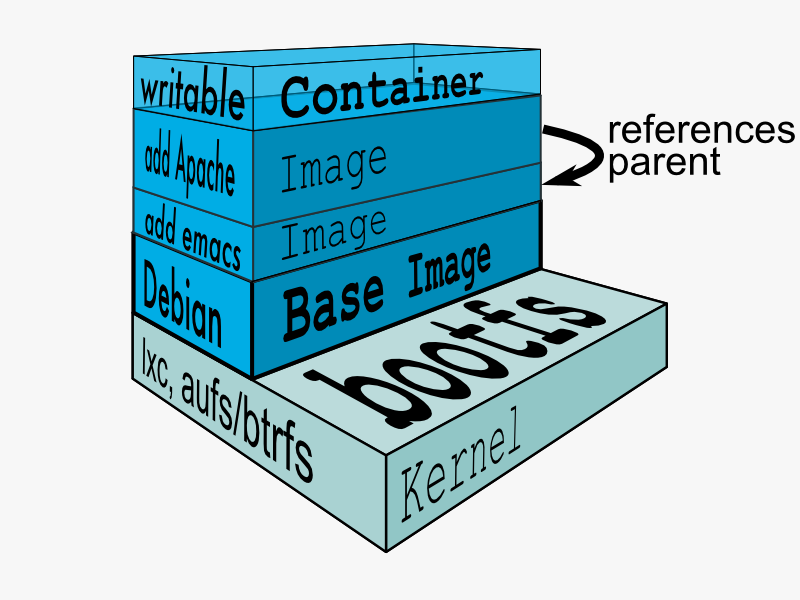
\includegraphics[width=.9\linewidth]{img/docker-filesystems-multilayer.png}.
\subsubsection{Union file system}
\label{sec-2-5-1}

At first, the top read-write layer has nothing in it, but any time a process creates a file, this happens in the top layer. And if something needs to update an existing file in a lower layer, then the file gets copied to the upper layer and changes go into the copy. The version of the file on the lower layer cannot be seen by the applications anymore, but it is there, unchanged. We call the union of the read-write layer and all the read-only layers a \textbf{union file system}.
\subsubsection{Base Image}
\label{sec-2-5-2}

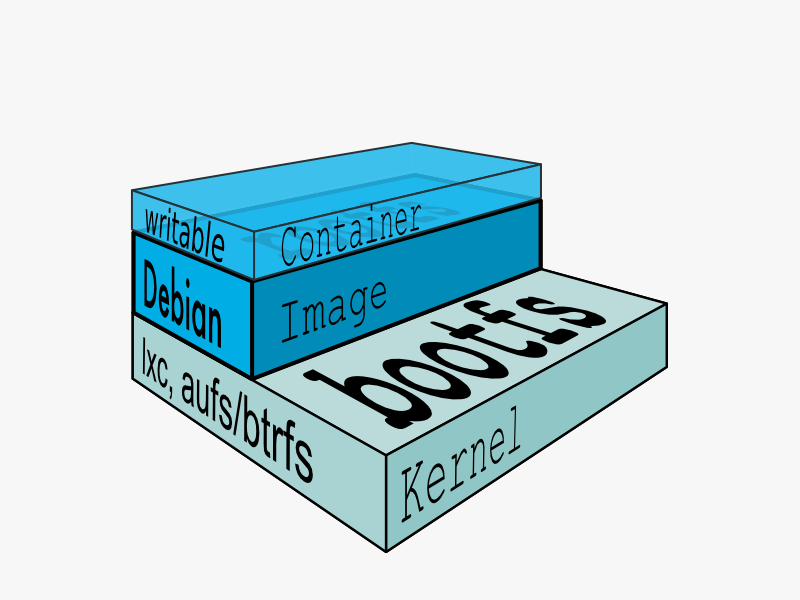
\includegraphics[width=.9\linewidth]{img/docker-filesystems-debianrw.png}
In Docker terminology, a read-only Layer is called an image. An image never changes.
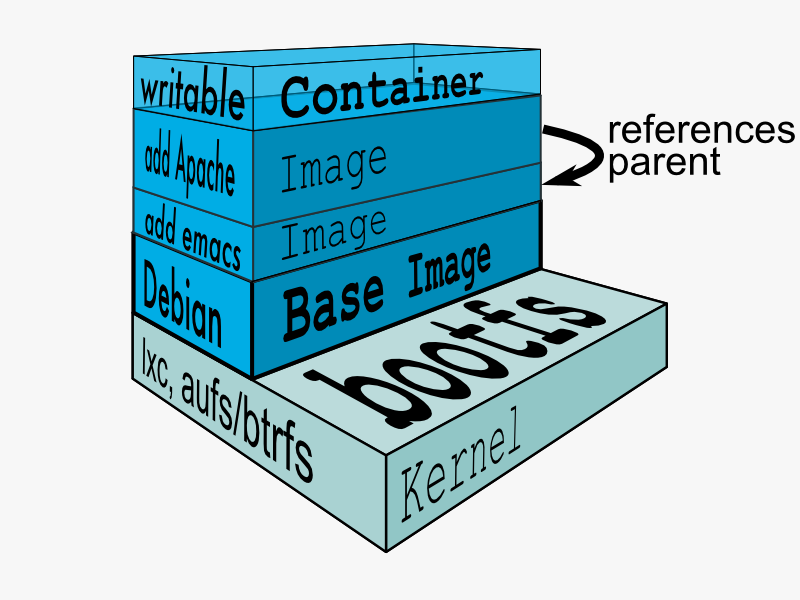
\includegraphics[width=.9\linewidth]{img/docker-filesystems-multilayer.png}
Each image may depend on one more image which forms the layer beneath it. We sometimes say that the lower image is the parent of the upper image. An image that has \textbf{no parent} is a \textbf{base image}.
All images are identified by a 64 hexadecimal digit string (internally a 256bit value). To simplify their use, a short ID of the first 12 characters can be used on the command line. There is a small possibility of short id collisions, so the docker server will always return the long ID.
\subsection{Container and Images}
\label{sec-2-6}

As \emph{Docker} is under heavy development, the file system storing \emph{Docker} related information changes rapidly. The main directory to look for \emph{Docker} relevant bits and bytes is \emph{var/lib/docker}. In this section \textbf{GUID} is the full blown container id as given by \texttt{docker ps -a -no-trunc}.
\subsubsection{LXC configuration}
\label{sec-2-6-1}

Using the Linux Container package \href{file://./lxc/}{http://linuxcontainers.org/}, \emph{Docker} configures each container partly by setting lxc options in \emph{var/lib/docker/container/GUID/config.lxc}. 
\subsubsection{Container Root File System}
\label{sec-2-6-2}

The corresponding root file system is stored in \emph{var/lib/docker/devicemapper/mnt/GUID/rootfs}.
Here GUID is the full blown container id as given by \texttt{docker ps -a -no-trunc}  
\subsubsection{Container Volumes}
\label{sec-2-6-3}

    If a container mounts a volume from inside the files on that volume are stored under \emph{var/lib/docker/vfs/dir/GUID}. Data stored under these volumes are persistent between container runs. There is a way to share these volumes between containers. 
\subsubsection{Removing a Container or an Image}
\label{sec-2-6-4}

To remove a container from a repository we list the containers and type:

\begin{verbatim}
docker ps -a
docker rm GUID
\end{verbatim}
To remove an image from a repository we list the images and type:

\begin{verbatim}
docker images -a
docker rmi USER/REPO:TAG
\end{verbatim}
Here \texttt{USER/REPO:TAG} referes to the user part, the repository part and the tag part of a special image. Note that command \texttt{docker images -a} my list the same GUID multiple times as the same image may be tagged differently. Removing an image beeing tagged multiple times only results in deleting the tag, keeping the other tagged version(s) in the repository.   
\section{Private Repositories}
\label{sec-3}

Right now (version 0.6), private repositories are only possible by hosting \href{https://github.com/dotcloud/docker-registry}{your private registry}. 
\subsection{Pushing to a private repo}
\label{sec-3-1}

To push or pull to a repository on your own registry, you must prefix the tag with the address of the registry’s host, like this:

\begin{verbatim}
# Tag to create a repository with the full registry location.
# The location (e.g. localhost.localdomain:5000) becomes
# a permanent part of the repository name
sudo docker tag 0u812deadbeef localhost.localdomain:5000/repo_name
# Push the new repository to its home location on localhost
sudo docker push localhost.localdomain:5000/repo_name
\end{verbatim}
The last command will fails, if no registry server answers locally on port 5000.
\subsection{Building a private repo}
\label{sec-3-2}

As \href{http://blog.docker.io/2013/07/how-to-use-your-own-registry/}{Sam Alba}, a Dotcloud.io engineer since the first beginning of \emph{docker} describes, we can build a registry container, provided \texttt{gunicorn} and \texttt{pip} is installed:

\begin{verbatim}
#install pip 
sudo apt-get install python-pip
#install gunicorn
sudo apt-get install gunicorn
#install the docker-registry container an run it
git clone https://github.com/dotcloud/docker-registry.git
cd docker-registry
cp config_sample.yml config.yml
sudo pip install -r requirements.txt
gunicorn --access-logfile - --log-level debug --debug \
    -b 0.0.0.0:5000 -w 1 wsgi:application
\end{verbatim}

To simplify things, the github repository comes with a Dockerfile do build a container from Ubuntu 13.4.
Once a repository has your registry’s host name as part of the tag, you can push and pull it like any other repository, but it will not be searchable (or indexed at all) in the Central Index, and there will be no user name checking performed. Your registry will function completely independently from the Central Index.
\subsection{Changes to the repository building code}
\label{sec-3-3}

The code posted by Sam Alba did not work out of the box neither on a Debian Wheezy (7.4) nor on an Ubuntu 12.4. We had to previously install and upgrade these packages on a docker host to get the \emph{gunicorn} application or the registry container running:
\subsubsection{Upgrade \emph{pip}}
\label{sec-3-3-1}


\begin{verbatim}
wgethttps://raw.github.com/pypa/pip/master/contrib/get-pip.py -o get-pip.py
sudo python get-pip.py
\end{verbatim}
\subsubsection{Install \emph{gcc}}
\label{sec-3-3-2}


\begin{verbatim}
sudo apt-get install -y gcc
\end{verbatim}
\subsubsection{Install deb-packages from file \emph{docker-registry/Dockerfile}}
\label{sec-3-3-3}


\begin{verbatim}
sudo apt-get install -y  git-core build-essential python-dev \
    libevent-dev python-openssl liblzma-dev wget
\end{verbatim}
\subsection{Registry as a  gunicorn application}
\label{sec-3-4}


\begin{verbatim}
git clone https://github.com/dotcloud/docker-registry.git
cd docker-registry
cp config_sample.yml config.yml
sudo pip install -r requirements.txt
gunicorn --access-logfile - --log-level debug --debug \
    -b 0.0.0.0:5000 -w 1 wsgi:application
\end{verbatim}
Finallay the \emph{gnuicorn} application worked as expected.
\subsection{Registry as container}
\label{sec-3-5}

An alternative way is to build a registry container after we installed the necessary libraries on the docker host.

\begin{verbatim}
git clone https://github.com/dotcloud/docker-registry.git
cd docker-registry
sudo docker build -rm -t registry .
sudo docker run -d -p 5000:5000 registry
\end{verbatim}
This results in an image tagged \emph{registry} and a container running on the same docker host exposing port 5000.
\subsection{Testing the private registry}
\label{sec-3-6}

Let's say we have two hosts, registry.localdomain and host01.localdomain both beeing known by local DNS. We build our images on host01.localdomain and store them on registry.localdomain running the registry container on port 5000. 
\subsubsection{On host01.localdomain}
\label{sec-3-6-1}

After a successful build or a a commit we tag an image properly and push it onto registry: 

\begin{verbatim}
# what have we got?
host01>sudo docker images
REPOSITORY                           TAG                 IMAGE ID            CREATED             VIRTUAL SIZE
debian/jenkins                       jenkins             38332d781d61        2 minutes ago        699.4 MB
ubuntu                               13.10               9f676bd305a4        3 weeks ago         182.1 MB
ubuntu                               saucy               9f676bd305a4        3 weeks ago         182.1 MB

host01>sudo docker tag 38332d781d61 registry.localdomain:5000/debian/jenkins
host01>sudo docker images 
REPOSITORY                                  TAG                 IMAGE ID            CREATED             VIRTUAL SIZE
debian/jenkins                              jenkins             38332d781d61        2 minutes ago        699.4 MB
registry.localdomain:5000/debian/jenkins    jenkins             38332d781d61        2 minutes ago        699.4 MB
ubuntu                                      13.10               9f676bd305a4        3 weeks ago         182.1 MB
ubuntu                                      saucy               9f676bd305a4        3 weeks ago         182.1 MB

# push this image to the registry server
host01>sudo docker push registry.localdomain:5000/debian/jenkins
The push refers to a repository [registry.localdomain:5000/debian/jenkins] (len: 1)
Sending image list
Pushing repository registry.localdomain:5000/debian/jenkins (1 tags)
11ed3d47ec89: Image successfully pushed 
38332d781d61: Image successfully pushed 
Pushing tag for rev [38332d781d61] on {http://registry.localdomain:5000/v1/repositories/debian/jenkins/tags/latest}

# remove both "images" locally
host01>sudo docker rmi  debian/jenkins
Untagged:38332d781d616823aaaaadc7c9ca4243f696b4efe2a74a49eb18fd062633198d
host01>sudo docker rmi registry.localdomain:5000/debian/jenki
Untagged:38332d781d616823aaaaadc7c9ca4243f696b4efe2a74a49eb18fd062633198d
# check for local images
host01>sudo docker images
REPOSITORY                         TAG                 IMAGE ID            CREATED             VIRTUAL SIZE
ubuntu                             13.10               9f676bd305a4        3 weeks ago         182.1 MB
ubuntu                             saucy               9f676bd305a4        3 weeks ago         182.1 MB

# no more local images for jenkins build: so we pull them from registry
# using the same command as the pull:
host01>sudo docker registry.localdomain:5000/debian/jenkin
Pulling repository host01.localdomain:5000/debian/jenkins
38332d781d61: Download complete 
9f676bd305a4: Download complete

#check the local images
host01>sudo docker images
REPOSITORY                                  TAG                 IMAGE ID            CREATED             VIRTUAL SIZE
registry.localdomain:5000/debian/jenkins    jenkins             38332d781d61        2 minutes ago       699.4 MB
ubuntu                                      13.10               9f676bd305a4        3 weeks ago         182.1 M
\end{verbatim}
\subsubsection{Web Services}
\label{sec-3-6-2}

\href{https://quay.io/}{quay.io} serves private registry the web, \href{https://index.docker.io/}{docker.io} provides a public index server.
\section{Installing a \emph{Scala/Java} WebApp}
\label{sec-4}

As a proof of concept, we install a \emph{Scala} WebApp with \emph{Lift}. We need \emph{Java} version > 6 and we use \emph{Lift} as the framework. 
\subsection{Installing the necessary packages and \emph{Java}}
\label{sec-4-1}

We need \emph{jdk} at least version 6, \emph{wegt}, \emph{zip} and git:

\begin{verbatim}
$ apt-get update
$ apt-get install -y apt-utils
$ apt-get install -y openjdk-7-jre
$ apt-get install -y openjdk-7-jdk
$ apt-get install -y wget
$ apt-get install -y zip
$ apt-get install -y git
\end{verbatim}
This installs Java 7 and my take a minute.
\subsection{Installing \emph{tomcat7}}
\label{sec-4-2}

We use \emph{tomcat} as the \textbf{Apache Tomcat Servlet/JSP} engine to serve our \emph{Scala} WebApp, installing it by typing:

\begin{verbatim}
$ apt-get update
$ apt-get install -y tomcat7
\end{verbatim}
Tomcat serves servlets  at \href{http://localhost:8080}{http://localhost:8080}. The debian package starts the service automatically at boot time via \emph{etc/init.d/tomcat7} script.
\subsection{Scala WebApp}
\label{sec-4-3}
\subsubsection{Installation}
\label{sec-4-3-1}

We download and configure a sample \emph{Scala} WebApp and unzip it under \emph{opt}.

\begin{verbatim}
$ wget -O /tmp/master.zip https://github.com/Lift/Lift_26_sbt/archive/master.zip
$ unzip -d /opt/ /tmp/master.zip
\end{verbatim}
\subsubsection{Compiling the WebApp}
\label{sec-4-3-2}

The first time this process may take several minutes to download \emph{maven} and the \emph{Scala}-files. Later calls only compile the relevant jar- and war-files. To compile the WebApp we type:

\begin{verbatim}
$  cd /opt/lift_26_sbt-master/scala_210/lift_basic/ && ./sbt compile
\end{verbatim}

\href{http:///Lift/web.net/getting_started}{/Lift/ web framework}  will download \emph{sbt}, \emph{Scala} and the necessary dependencies and compile the War-File \textbf{/opt/lift\_26\_sbt-master/scala\_210/lift\_basic/target/scala-2.10/lift-2.6-starter-template$_2$.10-0.0.3.war}. 
 
By typing \texttt{/opt/lift\_26\_sbt-master/scala\_210/lift\_basic/sbt  start} we should be able to see the WebApp at \href{http://localhost:8080}{http://localhost:8080}. To exit just type \texttt{exit}. The source of this WebApp is under \textbf{/opt/lift\_26\_sbt-master/scala\_210/lift\_basic/src/main/webapp/}. To prove the concept, we will later just change \emph{index.html}.
\subsection{Deploying the WebApp to \emph{tomcat7}}
\label{sec-4-4}

\emph{Lift} uses \emph{sbt} to compile the project and output a WAR- or JAR-file, which we want to copy into \emph{tomcat7}'s webapp directory \textbf{/var/lib/tomcat7/webapps/}. We recompile the package and deploy it statically into \emph{tomcat}.

\begin{verbatim}
$ cd /opt/lift_26_sbt-master/scala_210/lift_basic/
$  ./sbt  package
$ cp  target/scala-2.10/lift-2.6-starter-template_2.10-0.0.3.war \
    /var/lib/tomcat7/webapps/lift.war
$ service tomcat7 restart
\end{verbatim}
This copies the war-file and restarts \emph{tomcat7}. To see the WebApp direct your browser to \href{http://localhost:8080/lift_basic/}{http://localhost:8080/lift\_basic/}. There is no need to restart \emph{tomcat} manually, as the \emph{autoDeploy} attribute is set to ``true'' in file \textbf{/etc/tomcat7/server.xml}. \emph{tomcat} even unpacks war-files if attribute \emph{unpackWARs} is set to ``true''.
\subsection{Building a container with the WebApp}
\label{sec-4-5}
\subsubsection{The Dockerfile}
\label{sec-4-5-1}

The command 

\begin{verbatim}
sudo docker build -rm -t USER/REPO:TAG docker-dir/
\end{verbatim}
builds the WebApp container using the docker file inside \texttt{docker-dir/} and pushes it into repository \texttt{USER/REPO} with tag \texttt{TAG}. Creating directories for each docker file, we can split building the image into different tasks. This eases testing of the \texttt{RUN} commands inside the docker files. 
\begin{itemize}
\item \texttt{01\textbackslash{}\_openjdk7/Dockerfile} creates an image with \emph{Java} and some utilities installed.
\item \texttt{02\textbackslash{}\_tomcat7/Dockerfile} installs \emph{tomcat7} as the servlet engine.
\item \texttt{03\textbackslash{}\_install\textbackslash{}\_scala/Dockerfile} installs \emph{Scala} and compiles a sample WebApp.
\item \texttt{04\textbackslash{}deploy\textbackslash{}\_scala/Dockerfile}  compiles the sample WebApp and copies the war-file into \emph{tomcat7} webapp directory.
\end{itemize}

Note that each step in the installation process expects the previous image to be tagged properly. This can be avoided by concatenating the \texttt{RUN} commands from all the docker files into one single file.
\subsubsection{Starting the container}
\label{sec-4-5-2}

The sample WebApp gets served by the \emph{tomcat7} instance on port 8080. In order to expose this container port by the docker host we run the container  typing:

\begin{verbatim}
sudo docker run -i -t -p :8080:8080 USER/REPO:TAG /bin/bash
\end{verbatim}
\section{Jenkins}
\label{sec-5}

This section describes how to install a \emph{Jenkins} server, as described in \href{https://wiki.jenkins-ci.org/display/JENKINS/Installing%2BJenkins%2Bon%2BUbuntu}{https://wiki.jenkins-ci.org}. 
\subsection{Installation}
\label{sec-5-1}

On Debian-based distributions, such as \emph{Ubuntu}, you can install \emph{Jenkins} through \texttt{apt-get}. Recent versions are available in an apt repository. Older but stable LTS versions are in this apt repository.

You need to have a JDK and JRE installed. openjdk-7-jre and openjdk-7-jdk are suggested. As root we type

\begin{verbatim}
wget -q -O - http://pkg.jenkins-ci.org/debian/jenkins-ci.org.key \
 | sudo apt-key add - 
echo deb http://pkg.jenkins-ci.org/debian binary/ >  /etc/apt/sources.list.d/jenkins.list
apt-get update
apt-get install -y net-tools
apt-get install jenkins
\end{verbatim}

What does this package do?

\begin{itemize}
\item \emph{Jenkins} will be launched as a daemon up on start. See /etc/init.d/jenkins for more details.
\item The `jenkins' user is created to run this service.
\item Log file will be placed in \emph{var/log/jenkins/jenkins.log}. Check this file if you are troubleshooting Jenkins.
\item \emph{etc/default/jenkins will capture configuration parameters for the launch. - By default, /Jenkins} listen on port 8080. Access this port with your browser to start configuration.
\end{itemize}
\subsection{Configure Jenkins}
\label{sec-5-2}

We want to run \emph{Jenkins} on port 8090: 

\begin{verbatim}
sed -i s/HTTP_PORT=8080/HTTP_PORT=8090/ /etc/default/jenkins
\end{verbatim}
\subsection{Build a container and publish it into the registry}
\label{sec-5-3}

Each time the WebApp has changed in git, \emph{Jenkins} builds a new container,  consisting of three parts:
\begin{enumerate}
\item Deploying the WebApp-Files into the latest container.
\item Commit the newly build container and tag it properly.
\item Start the newly tagged container.
\end{enumerate}

We start this container, exposing port 8090:

\begin{verbatim}
sudo docker run -p :8090:8090 -i -t GUID /bin/bash
\end{verbatim}
\subsection{\textbf{TODO}}
\label{sec-5-4}

\begin{itemize}
\item jenkins startup errors with: ``  jenkins/etc/init.d/jenkins: line 108: ulimit: open files: cannot modify limit: Operation not permitted''
\item jenkins setup
\item jenkins web app source controll
\item start service \emph{jenkins} automatically
\end{itemize}
\subsection{Launch the newly build container}
\label{sec-5-5}
\section{Conclusion}
\label{sec-6}

On our test machines we could install a sample \emph{Scala} WebApp, register the source code with \emph{Jenkins} and get \emph{Jenkins} build a docker container each time the source code changed in \emph{git}. As a private registry server does not index the images, proper tagging is essential to pulling the proper container image. Once the image is pulled, it is indexed locally.

We recommend \emph{docker} as a robust and convenient virtualization tool that creates immutable images and speeds up software development and deployment.  
\section{Open Questions}
\label{sec-7}
\subsection{Networking}
\label{sec-7-1}
\subsection{Logging}
\label{sec-7-2}
\subsection{Persistence}
\label{sec-7-3}

 

\end{document}
